\section{Design and Solution}
\subsection{System Overview}
The core functionality of the system revolves around the following major components:

\begin{itemize}
    \item \textbf{Signal Processing and Control:} The system handles two primary signal sources:
    \begin{itemize}
        \item An NE555 timer circuit generating a PWM signal on PA1, with its frequency controlled through a feedback loop
        \item A function generator providing an external square wave input signal on PA2 for frequency measurement
        \item Signal switching between sources implemented through interrupt-driven control on PA0
    \end{itemize}

    \item \textbf{Analog Interface System:} The implementation includes:
    \begin{itemize}
        \item A 12-bit ADC continuously polling a potentiometer on PA5, with configurable sampling time and continuous conversion mode
        \item A 12-bit DAC on PA4 generating control voltages (0-3.3V) to modulate the 4N35 optocoupler
        \item Real-time conversion of ADC values to resistance measurements (0-5000~$\Omega$ range)
    \end{itemize}

    \item \textbf{Timer and Interrupt System:} The design features:
    \begin{itemize}
        \item TIM2 configured for precise frequency measurements using overflow detection
        \item EXTI interrupts on PA0, PA1, and PA2 for mode switching and edge detection
        \item Interrupt-driven frequency calculation using system clock references
    \end{itemize}

    \item \textbf{User Interface Components:} The system provides:
    \begin{itemize}
        \item An SSD1306 OLED display interfaced via SPI, showing current measurements
        \item A user button with debouncing for switching between measurement modes
        \item Real-time updates of both resistance and frequency measurements
    \end{itemize}
    \item \textbf{Critical Hardware Connections:} The system utilizes specific pin assignments:
    \begin{itemize}
        \item PA0: USER button interrupt handling (EXTI0)
        \item PA1: NE555 timer signal measurement (EXTI1)
        \item PA2: Function generator frequency measurement (EXTI2)
        \item PA4: DAC output for optocoupler control
        \item PA5: ADC input for potentiometer measurement
        \item PB3-PB7: SPI and control signals for OLED display
    \end{itemize}
\end{itemize}

% Path to block diagram figure
\begin{figure}[tbph]
  \centering
  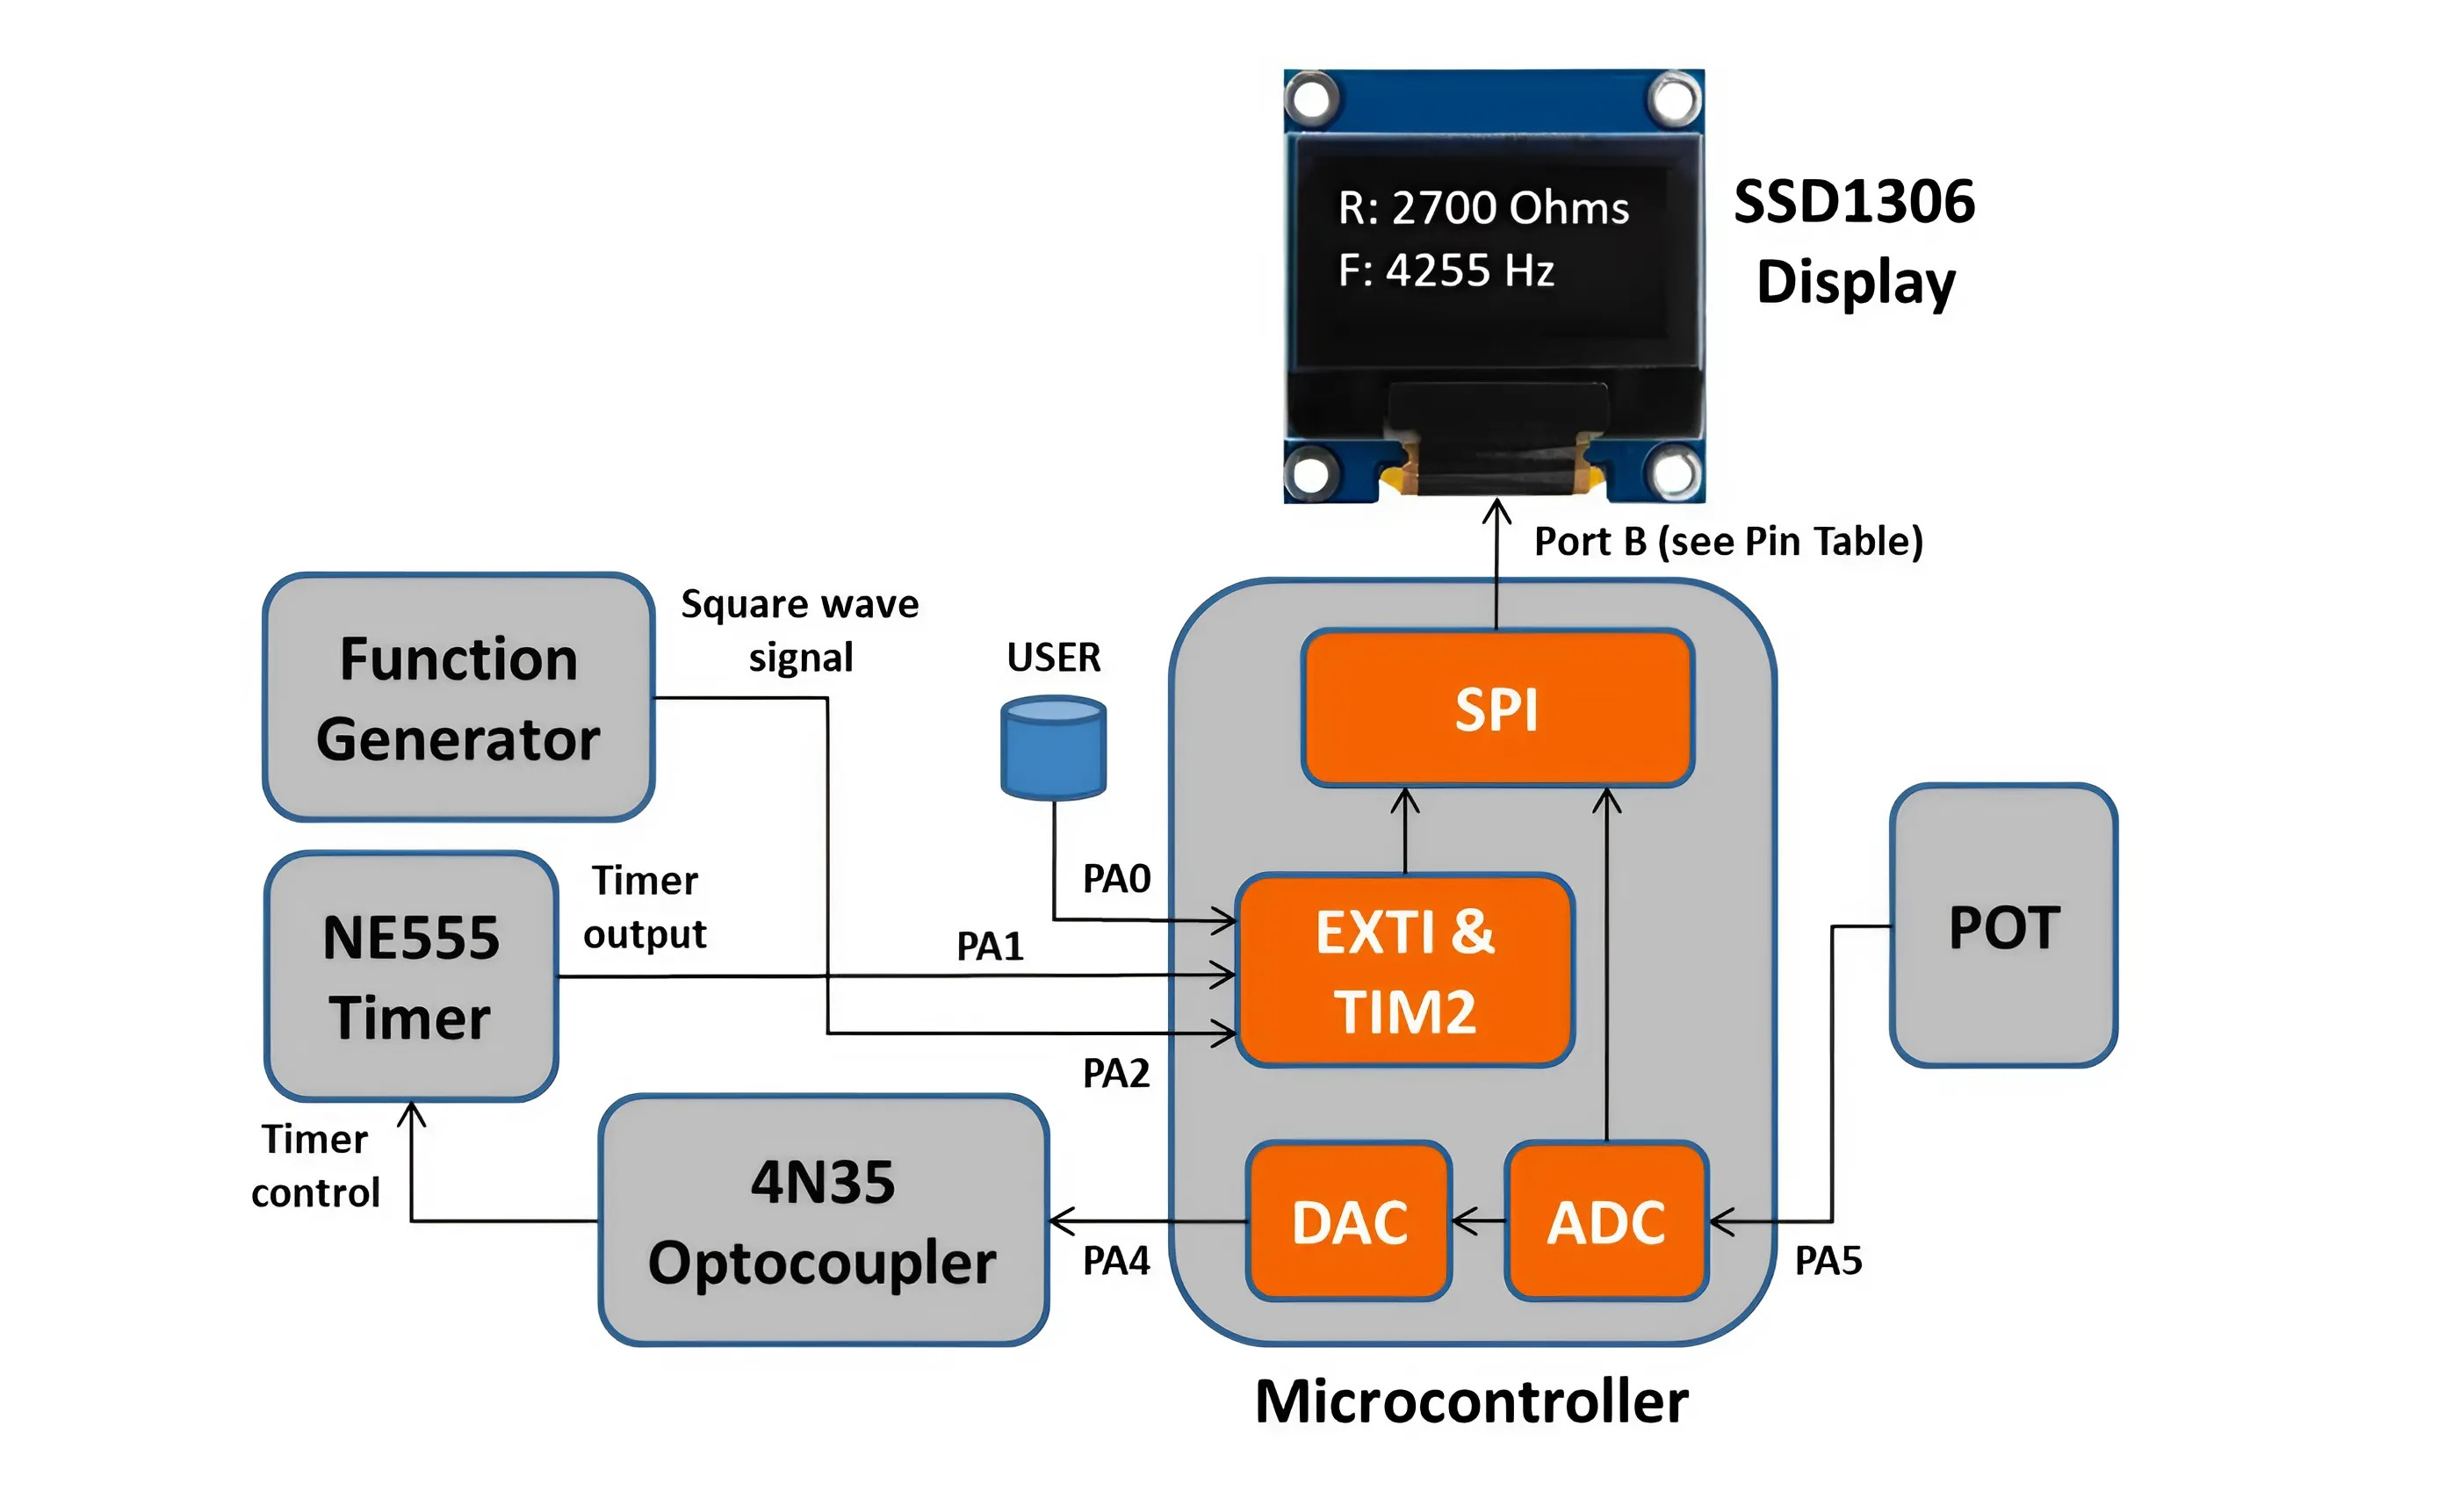
\includegraphics[width=0.7\linewidth]{graphics/system_blocks}
  \caption{System architecture showing the interaction between major components of the frequency measurement and signal generation system}
  \label{fig:systemblocks}
\end{figure}

\subsection{Hardware Design}
\subsubsection{Block Diagram}
%\begin{center}
%    \includegraphics[width=0.8\textwidth]{path_to_block_diagram.png} % Include your block diagram
%\end{center}

\subsubsection{Key Components and Connections}
\begin{itemize}[leftmargin=2em]
    \item \textbf{ADC Input:} Configured on pin PA5 for analog signal capture.
    \item \textbf{DAC Output:} Configured on pin PA4 for real-time output.
    \item \textbf{Mode-Switch Button:} External interrupt on pin PA0.
    \item \textbf{OLED Display:} SPI communication for real-time data visualization.
    \item \textbf{Power Supply:} Regulated 3.3V for stable operation.
\end{itemize}

\subsection{Software Design}
The software architecture includes:
\begin{itemize}[leftmargin=2em]
    \item \textbf{Initialization Functions:} Setting up system clocks and peripherals.
    \item \textbf{Interrupt Handlers:} Managing button presses for mode toggling (and others to be included).
    \item \textbf{Computation Algorithms:} Frequency and resistance calculations.
\end{itemize}

\subsubsection{Code Snippet: System Clock Initialization}
\begin{lstlisting}[caption=System Clock Initialization, label=lst:SystemClockInit]
void SystemClock48MHz(void) {
    RCC->CR &= ~(RCC_CR_PLLON);  // Disable PLL
    while ((RCC->CR & RCC_CR_PLLRDY) != 0);  // Wait for unlock
    RCC->CFGR = 0x00280000;  // Configure PLL
    RCC->CR |= RCC_CR_PLLON;  // Enable PLL
    while ((RCC->CR & RCC_CR_PLLRDY) != RCC_CR_PLLRDY);  // Lock PLL
    RCC->CFGR = (RCC->CFGR & (~RCC_CFGR_SW_Msk)) | RCC_CFGR_SW_PLL; // Switch clock
    SystemCoreClockUpdate();
}
\end{lstlisting}